\documentclass[doctor,proposal,color]{buaa}

\begin{document}

% Info
\thesistilte{\textcolor{red}{请在此处写各位同学的论文题目}}
\title{\buaaatthesistitle}
\authorname{研究生姓名}
\author{\buaaatauthorname}
\tutor{导师姓名}
\stuno{XXXX}
\major{专业名称}
\direction{研究方向}
\ckeyword{姿态估计、动作分割、行为识别、动作质量评估}
\ekeyword{Pose estimation, Action localization, Action recognition, Action quality assessment}

\hypersetup{
    bookmarksnumbered,
    bookmarksopen,
    pdftitle={\buaaatthesistitle},
    pdfauthor={\buaaatauthorname},
    pdfsubject={\buaaatuniversity \buaaatschool \buaaatdegree 研究生学位论文\buaaatdoctype},
    pdfcreator={LaTeXed~By~BUAA},
}

% Title_page(封面)
\pdfbookmark[0]{\buaaatthesistitle}{cover}
\maketitle
\linespread{1.5}
\pagestyle{frontmatter}

% Toc(目录)
\newpage
\phantomsection
\pdfbookmark[section]{\contentname}{contents}
\tableofcontents
\newpage
\phantomsection
\pdfbookmark[section]{\figurecontentname}{lof}
\listoffigures
% 模板暂无表格
%\newpage
%\phantomsection
%\pdfbookmark[section]{\tablecontentname}{lot}
%\listoftables
\newpage
\pagestyle{mainmatter}

% Main content
\section{论文研究背景与意义}

\subsection{论文选题背景}
参考文献引用:1)引文或转述观点最后一个句号之前用上标\upcite{yan2018spatial,wu2020comprehensive,hu2015,jdmsugg,lovell1999development};2)直接说明应与正文对齐,如文献\cite{yan2018spatial,wu2020comprehensive}。

\textbf{\color{red}(可以从如下几个方面进行论述:1、学术界理论研究背景,2、项目研究背景,3、实际应用背景)}

\subsection{研究现状概述}

针对本论文遇到的问题,XXX等人的方法存在XXXX问题。
\textbf{\color{red}
(用2页左右的篇幅,对文献综述所罗列的研究现状进行总结和分析,并列举与论文密切相关的几项工作)}


\subsection{研究目标与创新性}

\textbf{\color{red}(描述论文的目标以及成果,目标是解决什么问题/探索新的方向,成果可以是以下几种形式:1发表论文、2申请专利、3获得软件著作权、4开发装置、5开发软件模块或者系统、6构建一个数据集)}

针对XXX领域的不足,研究XXXX方法/开发XXX系统,解决XXX问题或者:探索XXX领域某方面的新思路。研究成果计划发表于XXX会议、申请XXX项发明专利、获得XXX项软件著作权、开发的软件系统将用于XXX、构建的数据集将在学术界公开。

\textbf{\color{red}(描述论文工作的创新性,与现有研究和工程方案的区别,侧重于理论方法研究的论文可以写方法思路的创新性,侧重于工程实践的论文,可以写系统方案、解决问题的新思路)}

论文将引入XXX思路、改进XXX方法、探索XXX理论,从而提高XXX准确率,实现XXX效果、解决XXX问题。
\section{研究内容与技术路线}

\textbf{\color{red}(用一段文字+图说明论文研究内容的设置情况,以及研究内容间的逻辑关系。逻辑关系可以是并列、先后,总分等)}

针对上述问题,本论文的工作分为如下几个方面,如\cref{fig_1}所示。首先研究XXX,在此基础上研究XXX,基于上述研究成果实现XXX。

\begin{figure}[h] 
	\centering
	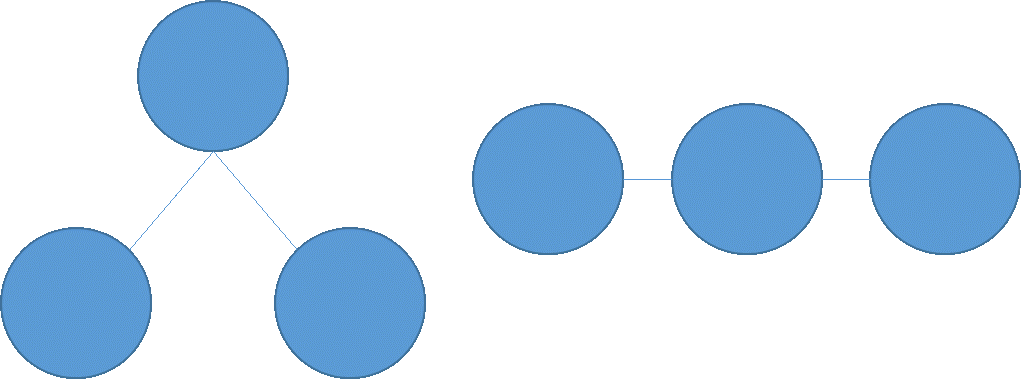
\includegraphics[width=0.4\linewidth]{fig_1.png} 
	\caption{研究内容关系示意图}
	\label{fig_1}
\end{figure}

\textbf{\color{red}(下面分别介绍每个研究内容)}


\subsection{研究内容一:xxxxxxxxx}

\subsection{研究内容二:xxxxxxxxx}

\subsection{研究内容三:xxxxxxxxx}

\textbf{\color{red}(下面通过图文的形式说明论文技术方案)}

\subsection{XXXXX方法技术路线}

本文使用XXX方法技术路线,如\cref{fig_2}所示。

\begin{figure}[h] 
	\centering
	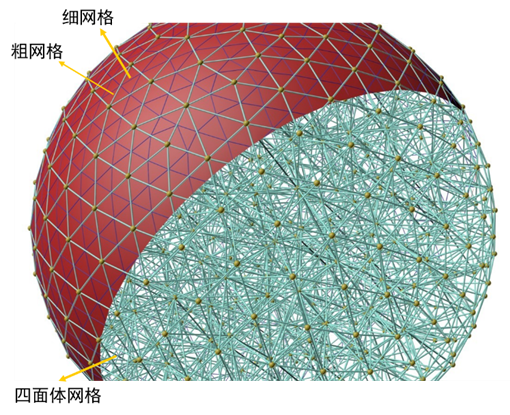
\includegraphics[width=0.6\linewidth]{fig_2.png}
	\caption{本论文拟构建的物理仿真模型示意图}  
	\label{fig_2}
\end{figure}

\subsection{XXXXX方法技术路线}

\subsection{XXXXX方法技术路线}
\section{论文工作安排计划}

\subsection{工作进度安排}
\subsection{论文工作基础}


\textbf{\color{red}(在以下几个方面选择几个方面进行说明:1)收集或者准备的数据集、2)完成或者正在进行的调研工作;3)已完成或者正在进行的理论推导、4)已经完成或者正在进行的开发系统或软件模块、5)正在进行或者完成的实验与实验结果)}

\subsection{可能遇到的问题以及解决途径}
\textbf{\color{red}
(描述论文可能遇到理论证明、工程开发、核心算法不足、实验数据等方面困难以及应对措施)}

% References
\clearpage
\nocite{*}
\phantomsection
\addcontentsline{toc}{section}{\bibname}
\bibliography{Refs}

\end{document}